
%(BEGIN_QUESTION)
% Copyright 2007, Tony R. Kuphaldt, released under the Creative Commons Attribution License (v 1.0)
% This means you may do almost anything with this work of mine, so long as you give me proper credit

Calculate the necessary size ($C_v$, and also pipe size in inches) control valve to pass a maximum of 350 SCFM of pure ozone gas (specific gravity = 1.8) in this drinking water disinfection system, where enough ozone (O$_{3}$) is continuously bubbled through 3 feet of water to kill most harmful micro-organisms:

$$\includegraphics[width=15.5cm]{i01714x01.eps}$$

Assume an ozone generator outlet pressure of 120 inches water column (gauge pressure, not absolute), a temperature of 50$^{o}$ F, and negligible friction in the ozone piping.

\vskip 10pt

$C_v$ = \underbar{\hskip 50pt} \hskip 100pt Nominal pipe size = \underbar{\hskip 50pt} inches

\underbar{file i01714}
%(END_QUESTION)





%(BEGIN_ANSWER)

Deduct 2 points if calculated pipe size is correct but not rounded to nearest appropriate nominal pipe size.

\vskip 10pt

$C_v$ = \underbar{\bf 64.06} \hskip 50pt Nominal pipe size = \underbar{\bf 2} inch (1.601 inches calculated)

%(END_ANSWER)





%(BEGIN_NOTES)

{\bf This question is intended for exams only and not worksheets!}.

%(END_NOTES)


